\documentclass[12pt]{article}
\usepackage{blubird}
% has options [nodate, nosans, nofancy, nocolor, code]

% TITLE
\title{what is a hole?}
\author{blu}
\date{22 apr 2024} % do not use if [nodate] option enabled

\begin{document}
\maketitle
\tableofcontents

i'm doing this for free pizza sorry if this is bad lol 

\section{what is a hole?}
Question (for those not in algebraic topology): how many holes do the following objects have? 
\begin{itemize}
  \item coffee cup
  \item hole dug in the ground
  \item straw 
  \item sphere (hollow) 
  \item Klein bottle
\end{itemize}

\noindent Question: Counting holes is hard -- how does one tell if a space has a hole?


\section{finding holes using tiling triangles (simplicial homology)}
   From a study of planar graphs or polyhedra, one might recall the \tbf{Euler
   characteristic} -- for a graph $G$ with $V$ vertices, $E$ edges, and $F$ faces
   (including the ``outside'' if necessary) we have $\chi(G) = V - E + F$. For
   planar graphs and polyhedral graphs we know that $\chi(G)$ = 2.
  
   Let's do it with what will look like roughly the same graph on paper, but we'll
   play around with gluing various edges together in various ways.
   \begin{exercise}
     Identify as many of the following shapes as you can. A correct answer will be
     ``continuously deformable'' into the pictures shown -- they don't have to be
     exact matches! Vertices of the same color should also be thought of as being
     ``glued together.''
   \begin{center}
       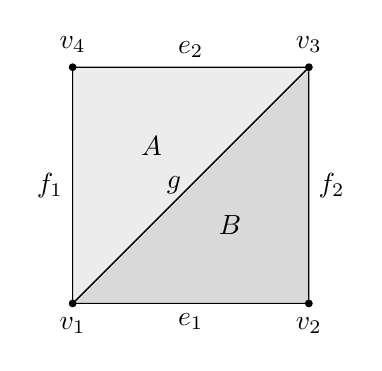
\begin{tikzpicture}
           \draw[fill=gray!30] (0,0) -- ++(3,0) -- ++(0, 3) -- ++(-3,-3) ;
          \node[circle,inner sep=1pt](D) at (2,1) {$B$};
          \draw[fill=gray!15] (0,0) -- ++(0,3) -- ++(3, 0) -- ++(-3,-3) ;
          \node[circle,inner sep=1pt](U) at (1,2) {$A$};
          \node[circle,fill,inner sep=1pt,label=below:$v_1$](p00) at (0,0) {};
          \node[circle,fill,inner sep=1pt,label=below:$v_2$](p10) at (3,0) {};
          \node[circle,fill,inner sep=1pt,label=above:$v_4$](p01) at (0,3) {};
          \node[circle,fill,inner sep=1pt,label=above:$v_3$](p11) at (3,3) {};
  
         \draw (p00) -- node[midway, above, left] {$g$} (p11);
         \draw (p00)  -- node[midway, below] {$e_1$} (p10) ;
         \draw (p01)  -- node[midway, above] {$e_2$} (p11) ;
         \draw (p00)  -- node[midway, left] {$f_1$} (p01) ;
         \draw (p10)  -- node[midway, right] {$f_2$} (p11) ;
       \end{tikzpicture}
       \begin{tikzpicture}
           \draw[fill=gray!30] (0,0) -- ++(3,0) -- ++(0, 3) -- ++(-3,-3) ;
          \node[circle,inner sep=1pt](D) at (2,1) {$B$};
          \draw[fill=gray!15] (0,0) -- ++(0,3) -- ++(3, 0) -- ++(-3,-3) ;
          \node[circle,inner sep=1pt](U) at (1,2) {$A$};
          \node[circle,fill,inner sep=1pt,label=below:$v_1$](p00) at (0,0) {};
          \node[circle,fill,inner sep=1pt,label=below:$v_2$](p10) at (3,0) {};
          \node[circle,fill,inner sep=1pt,label=above:$v_2$](p01) at (0,3) {};
          \node[circle,fill,inner sep=1pt,label=above:$v_3$](p11) at (3,3) {};
  
          \draw[-{Stealth[length=3mm, width=2mm]}, purple] (p00) -- node[midway, above, left] {$g$} (p11);
          \draw[-{Stealth[length=3mm, width=2mm]}, red] (p00)  -- node[midway, below] {$e$} (p10) ;
          \draw[-{Stealth[length=3mm, width=2mm]}, blue] (p01)  -- node[midway, above] {$f$} (p11) ;
          \draw[-{Stealth[length=3mm, width=2mm]}, red] (p00)  -- node[midway, left] {$e$} (p01) ;
          \draw[-{Stealth[length=3mm, width=2mm]}, blue] (p10)  -- node[midway, right] {$f$} (p11) ;
       \end{tikzpicture}
       \begin{tikzpicture}
           \draw[fill=gray!30] (0,0) -- ++(3,0) -- ++(0, 3) -- ++(-3,-3) ;
          \node[circle,inner sep=1pt](D) at (2,1) {$B$};
          \draw[fill=gray!15] (0,0) -- ++(0,3) -- ++(3, 0) -- ++(-3,-3) ;
          \node[circle,inner sep=1pt](U) at (1,2) {$A$};
          \node[circle,fill,inner sep=1pt,label=below:$v$](p00) at (0,0) {};
          \node[circle,fill,inner sep=1pt,label=below:$v$](p10) at (3,0) {};
          \node[circle,fill,inner sep=1pt,label=above:$v$](p01) at (0,3) {};
          \node[circle,fill,inner sep=1pt,label=above:$v$](p11) at (3,3) {};
         \draw[-{Stealth[length=3mm, width=2mm]}, purple] (p00) -- node[midway, above, left] {$g$} (p11);
         \draw[-{Stealth[length=3mm, width=2mm]}, red] (p00)  -- node[midway, below] {$e$} (p10) ;
         \draw[-{Stealth[length=3mm, width=2mm]}, red] (p01)  -- node[midway, above] {$e$} (p11) ;
         \draw[-{Stealth[length=3mm, width=2mm]}, blue] (p00)  -- node[midway, left] {$f$} (p01) ;
         \draw[-{Stealth[length=3mm, width=2mm]}, blue] (p10)  -- node[midway, right] {$f$} (p11) ;
      \end{tikzpicture}
  \end{center}
  \begin{center}
      \begin{tikzpicture}
          \draw[fill=gray!30] (0,0) -- ++(3,0) -- ++(0, 3) -- ++(-3,-3) ;
         \node[circle,inner sep=1pt](D) at (2,1) {$B$};
         \draw[fill=gray!15] (0,0) -- ++(0,3) -- ++(3, 0) -- ++(-3,-3) ;
         \node[circle,inner sep=1pt](U) at (1,2) {$A$};
         \node[circle,fill,inner sep=1pt,label=below:$v_2$](p00) at (0,0) {};
         \node[circle,fill,inner sep=1pt,label=below:$v_1$](p10) at (3,0) {};
         \node[circle,fill,inner sep=1pt,label=above:$v_1$](p01) at (0,3) {};
         \node[circle,fill,inner sep=1pt,label=above:$v_2$](p11) at (3,3) {};
 
        \draw[-{Stealth[length=3mm, width=2mm]}, purple] (p00) -- node[midway, above, left] {$g$} (p11);
        \draw[{Stealth[length=3mm, width=2mm]}-, red] (p00)  -- node[midway, below] {$e$} (p10) ;
        \draw[-{Stealth[length=3mm, width=2mm]}, red] (p01)  -- node[midway, above] {$e$} (p11) ;
        \draw[{Stealth[length=3mm, width=2mm]}-, blue] (p00)  -- node[midway, left] {$f$} (p01) ;
        \draw[-{Stealth[length=3mm, width=2mm]}, blue] (p10)  -- node[midway, right] {$f$} (p11) ;
      \end{tikzpicture}
      \begin{tikzpicture}
          \draw[fill=gray!30] (0,0) -- ++(3,0) -- ++(0, 3) -- ++(-3,-3) ;
         \node[circle,inner sep=1pt](D) at (2,1) {$B$};
         \draw[fill=gray!15] (0,0) -- ++(0,3) -- ++(3, 0) -- ++(-3,-3) ;
         \node[circle,inner sep=1pt](U) at (1,2) {$A$};
         \node[circle,fill,inner sep=1pt,label=below:$v$](p00) at (0,0) {};
         \node[circle,fill,inner sep=1pt,label=below:$v$](p10) at (3,0) {};
         \node[circle,fill,inner sep=1pt,label=above:$v$](p01) at (0,3) {};
         \node[circle,fill,inner sep=1pt,label=above:$v$](p11) at (3,3) {};
 
        \draw[-{Stealth[length=3mm, width=2mm]}, purple] (p00) -- node[midway, above, left] {$g$} (p11);
        \draw[-{Stealth[length=3mm, width=2mm]}, red] (p00)  -- node[midway, below] {$e$} (p10) ;
        \draw[-{Stealth[length=3mm, width=2mm]}, red] (p01)  -- node[midway, above] {$e$} (p11) ;
        \draw[-{Stealth[length=3mm, width=2mm]}, blue] (p00)  -- node[midway, left] {$f$} (p01) ;
        \draw[{Stealth[length=3mm, width=2mm]}-, blue] (p10)  -- node[midway, right] {$f$} (p11) ;
      \end{tikzpicture}
 
  \end{center}
\end{exercise}

  \noindent Keep these in mind! They will be our ``prototypical examples'' going
  forward.
 
  How do you argue that the spaces that these graphs represent are
  \tit{not isomorphic} to the normal plane $\RR^2$? One way is with the
  Euler characteristics of all of these graph representations:
    \begin{center}
      \begin{tabular}{c|ccccc}
        $G$ & (A) & (B) & (C) & (D) & (E) \\ \hline
        shape & $[0,1]^2$ & $S^2$ & $\TT^2$ & $\RR P^2$ & $K$ \\
        $\chi(G)$ & 2 & 2 & 0 & 1 & 0
      \end{tabular}
    \end{center}
    Note that the Euler characteristic isn't quite enough to differentiate the
  surfaces depicted above -- after all, we only have one number. Let's really use
  the structure of the graph now to analyze these surfaces at each dimension.
 
  First, for every top-dimensional triangular (simplicial) face (here,
  2-dimensional), let's order the vertices so that when we do our gluing, the
  orientation of the edges that are glued are consistent with the ordering of the
  vertices. As an example:
    \begin{center}
 
      \begin{tikzpicture}
          \draw[fill=gray!30] (0,0) -- ++(3,0) -- ++(0, 3) -- ++(-3,-3) ;
         \node[circle,inner sep=1pt](D) at (2,1) {$B$};
         \draw[fill=gray!15] (0,0) -- ++(0,3) -- ++(3, 0) -- ++(-3,-3) ;
         \node[circle,inner sep=1pt](U) at (1,2) {$A$};
         \node[circle,fill,inner sep=1pt,label=below:$v \, (0 / 0)$](p00) at (0,0) {};
         \node[circle,fill,inner sep=1pt,label=below:$v \, (1)$](p10) at (3,0) {};
         \node[circle,fill,inner sep=1pt,label=above:$v \, (1)$](p01) at (0,3) {};
         \node[circle,fill,inner sep=1pt,label=above:$v \, (2 / 2)$](p11) at (3,3) {};
 
        \draw[-{Stealth[length=3mm, width=2mm]}, purple] (p00) -- node[midway, above, left]        {$g$} (p11);
        \draw[-{Stealth[length=3mm, width=2mm]}, red] (p00)  -- node[midway, below] {$e$}          (p10) ;
        \draw[-{Stealth[length=3mm, width=2mm]}, red] (p01)  -- node[midway, above] {$e$}          (p11) ;
        \draw[-{Stealth[length=3mm, width=2mm]}, blue] (p00)  -- node[midway, left] {$f$}          (p01) ;
        \draw[-{Stealth[length=3mm, width=2mm]}, blue] (p10)  -- node[midway, left] {$f$}          (p11) ;
      \end{tikzpicture}
    \end{center}
  In general, we might have an $n$-dimensional \tbf{simplex} as a part of our
  space $G$, which we define as a continuous image of the canonical $n$-simplex
  $\Delta^n = \set{\bf x \in \RR^{n+1} : \sum_{i=1}^{n+1} x_i = 1, x_i \geq
  0}$ into $G$, which we also write in terms of its vertices $[v_0, v_1,
  \dots, v_n]$. The relationship between dimensions is one of the
  \tbf{boundary} -- for instance, when we take an $n$-dimensional simplex of our
  space, its boundary is a union of $(n-1)$-simplices. With the orientation on each
  simplex, we define the \tbf{boundary map} acting on an $n$-simplex $\sigma$ to be the
  following formal sum of $n-1$-simplices:
  \[
  \bound \sigma = \sum_{i=0}^n (-1)^i \sigma\big|_{[v_0, v_1, \dots, v_{i-1},
  v_{i+1}, \dots, v_n]}
  \]
  The signs are maybe a surprising addition -- but with this, one can consider the
  integer linear combinations of all of the $k$-dimensional simplices $C_k(G)$ for
  one of our spaces, and the boundary maps assemble the $C_k$s into a \tbf{chain
  complex}:
  \[
    \dots \to C_n(G) \xto {\partial_n} \dots \to C_2(G) \xto{\partial_2} C_1(G)
    \xto{\partial_1} C_0(G) \xto{\partial_0} 0
  \]
  where we extend the boundary maps to act linearly on integer linear combinations
  of simplices.
 
  The key observation (due to Emmy N\"oether and Mayer/Vietoris) -- if the boundary of a           suitable sum of simplices is 0,
  these simplices encircle a closed region in $G$. But, if such a sum of
  simplices is not the boundary of any simplex in $G$, then we have
  detected a hole within our space! Therefore, the linear subspace of $C_n$
  that encircles closed regions in $G$ but ignoring any parts of it that actually
  do describe closed regions in $G$, gives us a subspace spanned by the
  holes of $G$! Interpreting this from the lens of linear
  algebra, we define the \tbf{homology groups}
  \[
  \boxed{H_n(G) = \frac{\ker \bound_n}{\im \bound_{n+1}}}
  \]
  As a fact to make these well-defined, we need to know that $\boxed{\bound^2 = 0}$, which
  is a defining feature of a general chain complex (that I've omitted until now).
  Now we can basically use linear algebra to compute them, since a basis of
  these subspaces tells us exactly where the holes are in our space at any
  dimension we like! This is the construct that will allow us to make more
  granular comparisons between spaces:
  \begin{center}
      \begin{tabular}{c|ccccc}
        $G$ & $S^2$ & $\TT^2$ & $\RR P^2$ & $K$ \\ \hline
        $H_0(G)$ & $\ZZ$ & $\ZZ$ & $\ZZ$ & $\ZZ$ \\
        $H_1(G)$ & $0$ & $\ZZ^2$ & $\ZZ / 2 \ZZ $ & $\ZZ \times \ZZ / 2\ZZ$ \\
        $H_2(G)$ & $\ZZ$ & $\ZZ$ & $0$ & $0$ \\
      \end{tabular}                                    
    \end{center}
 
  \begin{exercise}
  We can also recover the Euler characteristic from these groups! For a general
  topological space, the Euler characteristic is defined as $\chi(G) =
  \sum_{i=0}^\infty (-1)^i \dim_{\ZZ} H_i(G)$ (where the dimension here ignores
  any non-$\ZZ$ factors in the homology). Check this!
  \end{exercise}
 
  This construct isn't a panacea -- there are spaces that homology cannot tell
  apart. For instance, consider the space constructed by gluing a sphere and two
  circles together all at the same point. The homology of a torus/doughnut is
  identical to this! Other tools have to come into play to tell these spaces
  apart (cohomology, homotopy). However, homology is still very powerful!
  \begin{idea}
    Representing general (topological) spaces as graphs is very
  powerful and fairly general, and allows one to study them with algebraic tools.
  \end{idea}


\section{finding holes using functions and critical points (Morse homology)}
It turns out that on a smooth surface, another way one can detect holes is with
the help of looking at functions on it and their critical points. 

Suppose we have a smooth manifold $M$ and a function $f : M \to \RR$. In all of
the examples that follow, we
will let $M$ be immersed in Euclidean space and $f$ the projection onto a
coordinate. Again, we want to construct a \emph{chain complex} with this
information, and it turns out that we can do such a thing with the help of
critical points of $f$. Recall that critical points are points $p \in M$ such
that $df_p = 0$. We assume that all critical points are \emph{non-degenerate},
so that if we evaluate the Hessian $H(f, p)$, there are no zero eigenvalues of
the Hessian. 
\begin{definition*}
  The \emph{index} of a critical point $p$, $ind(p)$, is the number of
  \emph{negative} eigenvalues of $H(f, p)$. Let $crit_i(f)$ be the set of index
  $i$ critical points of $f$. 
\end{definition*}
We will consider the (negative) gradient flow of $f$, $- \grad f$, on $M$. This
gives a family of diffeomorphisms on $M$, $\psi: \RR \times  M \to M$, with
$\psi_0 = \id$, and $\dv{}t \psi_s = -\grad f$. 
\begin{definition*}
  For a critical point $p$, the \emph{descending and ascending manifolds} of $p$ are 
\[
  \mathcal D(p) = \set{x \in M : \lim_{s\to -\infty} \psi_s(x) = p}
\] 
\[
  \mathcal A(p) = \set{x \in M : \lim_{s\to +\infty} \psi_s(x) = p}
\]
You can think of this as the sets of points that have $p$ as a source vs. as a
sink, respectively. 
\end{definition*}
\begin{definition*}
  A \emph{flow line} from a critical point $p$ to a critical point $q$ is a path
  $\gamma : \RR \to M$ such that $\gamma'(s) = -\grad f(\gamma(s))$ (i.e. it
  lies tangent to the gradient flow), $\lim_{s\to \infty} \gamma(s) = q$,
  $\lim_{s\to -\infty} \gamma(s) = p$. 
\end{definition*}
Flow lines have an action of $\RR$ on them (it's the diffeomorphisms $\psi_s$,
acting by time-translation). 
\begin{definition*}
  $M(p, q)$ is the moduli space of flow lines from $p$ to $q$, up to
  translation. In other words, $M(p, q) = (\mathcal D(p) \cap \mathcal A(q)) /
  \RR$. This is a $(ind(p) - ind(q) - 1)$-dimensional manifold.
\end{definition*}
We also can orient $M(p, q)$. For each critical point $p$, orient the descending
manifold $\mathcal D(p)$. At any point in the image of $\gamma$, we have an
isomorphism, canonical at the level of orientations: 
\[
 T\mathcal D(p) \iso T(\mathcal D(p) \cap \mathcal A(q)) \oplus (TX / T\mathcal
 A(q)) \iso T_\gamma M(p, q) \oplus T\gamma \oplus T_q \mathcal D(q)
\]
We orient $\mathcal M(p, q)$ so that this isomorphism is orientation-preserving.

In general, $M(p, q)$ can be compactified with broken flow lines, where the
extra points added in consist of lines through critical points of lower index.  

\begin{definition*}
  The chain complex is defined by $C_i(f, g) = \ZZ crit_i(f)$, and the
  differential $\partial(p) = \sum_{q \in crit_{i-1}(f)} |M(p, q)| q$, where the
  number of points is counted with the correct orientation. 
\end{definition*}

\section{finding holes using differential forms (de Rham cohomology)}




\end{document} 
